  Электромагнитный калориметр является одной из основных частей детектора Belle II. Поскольку треть продуктов распада B-мезонов - это $\pi^0$ или другие нейтральные частицы, которые распадаются на фотоны в диапазоне энергий 20МэВ - 4ГэВ, и регистрируются электромагнитным калориметром, то требуется высокая разрешающая способность электромагнитного калориметра. В качестве сцинтилляционного кристаллического материала для калориметра Belle II был выбран CsI (Tl) из-за его высокого световыхода, относительно короткой длины излучения, хороших механических свойств и умеренной цены. Электромагнитный калориметр состоит из 8736 CsI (Tl) кристаллов и разделен на три части: передняя (Forward), задняя (Backward), а также цилиндрическая (Barrel) (Рис. 3).
Основными задачами калориметра являются\cite{TechRep}:
\begin{itemize}
  \item Регистрация фотонов и электронов
  \item Идентификация электронов
  \item Работа в широком диапазоне энергий 20 МэВ - 4 ГэВ в лабораторной системе отсчета
  \item Измерение светимости офлайн и онлайн
\end{itemize}\par
%\begin{wrapfigure}{l}{0.55\textwidth}
%  \begin{center}
%    \includegraphics[width=0.5\textwidth]{lom_connection.pdf}
%  \end{center}
%  \caption{Схема устройства триггерных ячеек в секторах и передача данных монитору светимости через FAM}
%\end{wrapfigure}
  Для регистрации сигнала с кристаллов на каждом из них установлено 2 фотодиода, которые преобразуют сцинтилляционное свечение в электрический сигнал, который поступает на вход предусилителей и преобразуется в импульс напряжения. Далее импульс напряжения поступает в модуль ShaperDSP, который осуществляет формирование, усиление сигнала, вычисляет амплитуду и время срабатывания счетчика. В каждый модуль ShaperDSP поступает сигнал с 8-16 кристаллов, образуя тем самым триггерную ячейку. Каждая торцевая секция разделена на 16 секторов, каждый сектор содержит две триггерные ячейки, данные с которых, проходя через ShaperDSP, передаются в модуль FAM. FAM суммирует сигналы с двух триггерных ячеек и передает аналоговую сумму сигналов на модуль онлайн монитора светимости (LOM) (Рис. 4).
\begin{figure}
\centering
\begin{minipage}[t]{.5\textwidth}
  \centering
  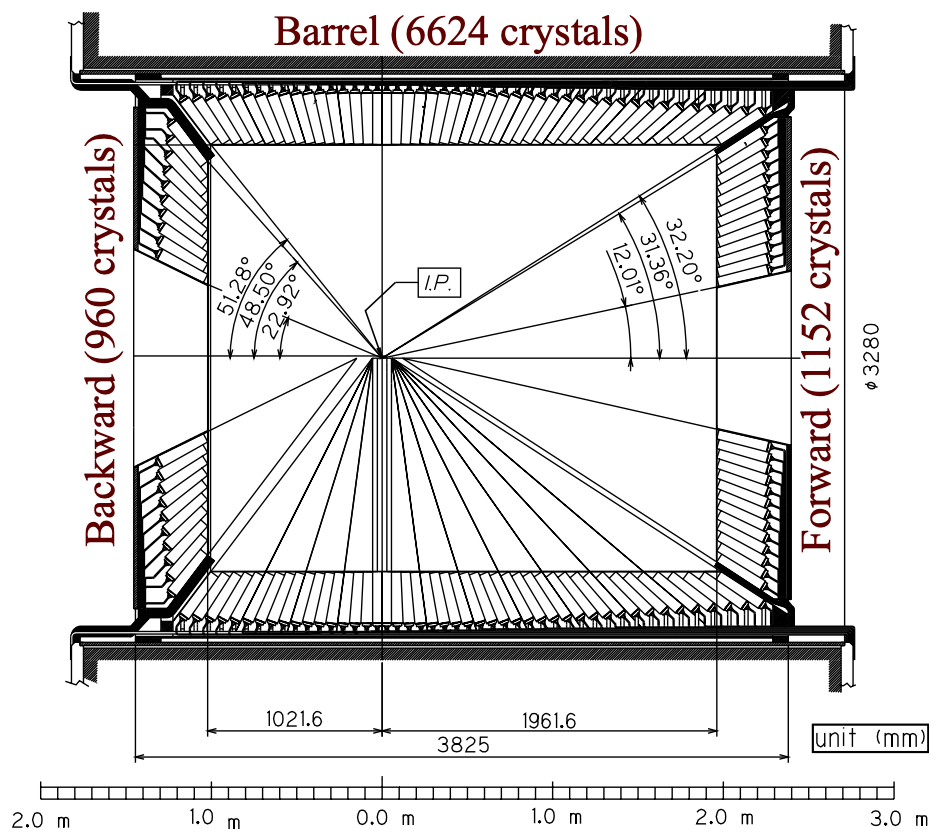
\includegraphics[width=.95\linewidth]{ECL}
  \caption{Срез электромагнитного калориметра (ECL).}
  \label{fig:test1}
\end{minipage}%
\begin{minipage}[t]{.5\textwidth}
  \centering
  \includegraphics[width=.95\linewidth, height=5cm]{lom_connection.pdf}
  \caption{Схема устройства триггерных ячеек в секторах и передача данных монитору светимости через FAM.}
  \label{fig:test2}
\end{minipage}
\end{figure}
